\section{Calculate the partial decay width for the decay \texorpdfstring{$\tau^- \to \pi^- \nu_\tau$}{tau- to pi- nu-tau} in the following steps.}

\textbf{a)}: Draw the Feynman diagram and snow that the corresponding matrix element is
\begin{align*}
    \mathcal{M} &= \sqrt{2}G_F f_\pi \bar{u}(p_\nu) \gamma^\mu \frac{1}{2}(1 - \gamma^5) u(p_\tau) g_{\mu\nu}p_\pi^\nu
\end{align*}

The Feynman diagram:
\begin{center}
    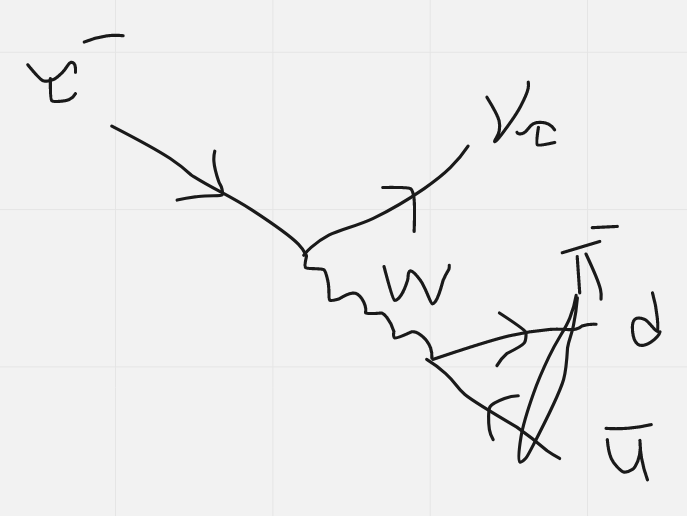
\includegraphics[width=0.5\textwidth]{q2a_diagram.png}
\end{center}

The parts:
\begin{itemize}
    \item Incoming $\tau^-$: $u(p_\tau)$
    \item Outgoing $\nu_\tau$: $\bar{u}(p_\nu)$
    \item $W^-$ propagator: $\frac{-i[g_{\mu\nu} - q_\mu q_\nu / m_W^2]}{q^2-m_W^2}$ (or appx $\frac{-ig_{\mu\nu}}{m_W^2}$)
    \item $\tau^- \to W^- \nu_\tau$ vertex: $\frac{-ig_W}{\sqrt{2}}\frac{1}{2}\gamma^\mu(1-\gamma^5)$
    \item Outgoing pion with the vertex: $\frac{-ig_W}{\sqrt{2}}\frac{1}{2}f_\pi p_\pi^\nu$
\end{itemize}

Put those all together:
\begin{align*}
    -iM_{fi} &= \bar{u}(p_\nu) \frac{-ig_W}{\sqrt{2}}\frac{1}{2}\gamma^\mu(1-\gamma^5) u(p_\tau) \frac{-ig_{\mu\nu}}{m_W^2}\frac{g_W}{\sqrt{2}}\frac{1}{2}f_\pi p_\pi^\nu \\
    M_{fi} &= \frac{1}{m_W^2}\frac{g_W}{\sqrt{2}}\frac{1}{2}f_\pi \frac{g_W}{\sqrt{2}}\bar{u}(p_\nu)\gamma^\mu\frac{1}{2}(1-\gamma^5) u(p_\tau) g_{\mu\nu} p_\pi^\nu \\
    &= \frac{g_W^2}{4m_W^2}f_\pi \bar{u}(p_\nu)\gamma^\mu\frac{1}{2}(1-\gamma^5) u(p_\tau) g_{\mu\nu} p_\pi^\nu \\
    &= \sqrt{2} G_F f_\pi \bar{u}(p_\nu)\gamma^\mu\frac{1}{2}(1-\gamma^5) u(p_\tau) g_{\mu\nu} p_\pi^\nu \\
\end{align*}

That last line came from $\frac{G_F}{\sqrt{2}} = \frac{g_W^2}{8m_W^2}$ (for low $q^2$).

\textbf{b)}: Taking the $\tau^-$ spin in the $z$-direction and the four-momentum of the neturino to be $p_\nu = p^*(1, \sin(\theta), 0, \cos(\theta))$, show that the leptonic current is $j^\mu = \sqrt{2m_\tau p^*}(-s,-c,-ic,s)$, where $s=\sin(\theta/2), c=\cos(\theta/2)$. For this configuration, the spinor for the $\tau^-$ can be taken to be $u_1$ for a particle at rest.

The leptonic current: $\bar{u}(p_\nu)\gamma^\mu\frac{1}{2}(1-\gamma^5) u(p_\tau)$. Make the approximation that chirality = helicity for high-energy particles like this.

We have $p_\nu = p^*(1, \sin(\theta), 0, \cos(\theta)), p_\tau = (m_\tau, 0, 0, 0)$, i.e. $s_\tau=0, c_\tau=1$

\begin{align*}
    \bar{u}(p_\nu)\gamma^\mu\frac{1}{2}(1-\gamma^5) u(p_\tau)
    &= \bar{u}(p_\nu)\gamma^\mu\frac{1}{2}(1-\gamma^5) u_1(p_\tau) \\
    &= \bar{u}(p_\nu)\gamma^\mu\frac{1}{2}(1-\gamma^5) \sqrt{E_\tau + m_\tau}\begin{pmatrix}
        1 \\ 0 \\ 0 \\ 0 \\
    \end{pmatrix} \\
    &= \bar{u}(p_\nu)\gamma^\mu\frac{1}{2}\begin{pmatrix}
        1 & 0 & -1 & 0\\
        0 & 1 & 0 & -1\\
        -1 & 0 & 1 & 0 \\
        0 & -1 & 0 & 1 \\
    \end{pmatrix} \sqrt{2m_\tau}\begin{pmatrix}
        1 \\ 0 \\ 0 \\ 0 \\
    \end{pmatrix} \\
    &= \sqrt{2m_\tau}\frac{1}{2}\bar{u}(p_\nu)\gamma^\mu\begin{pmatrix}
        1 \\
        0 \\
        -1 \\
        0 \\
    \end{pmatrix} \\
\end{align*}

For $u(p_\nu)$ we can use $u_\downarrow$ since we had $P_L$, and $\phi=0$ wlog since it's along the $z$ axis:

\begin{align*}
    \bar{u}(p_\nu) &= u_\downarrow(p_\nu)^\dagger \gamma^0\\
    &= \sqrt{E_\nu} \begin{pmatrix}
        -s \\
        c \\
        s \\
        -c \\
    \end{pmatrix}^\dagger \gamma^0\\
    &= \sqrt{p^*} \begin{pmatrix}
        -s &
        c &
        -s &
        c \\
    \end{pmatrix}\\
\end{align*}

Calculate some matrix products:
\begin{align*}
    \gamma^0u_1(p_\tau) &= \begin{pmatrix}
        1 & 0 & 0 & 0 \\
        0 & 1 & 0 & 0 \\
        0 & 0 & -1 & 0 \\
        0 & 0 & 0 & -1 \\
    \end{pmatrix}\begin{pmatrix}
        1 \\ 0 \\ -1 \\ 0 \\
    \end{pmatrix}\\
    &= \begin{pmatrix}
        1 \\
        0 \\
        1 \\
        0 \\
    \end{pmatrix}\\
    \begin{pmatrix}
        -s & c & -s & c \\
    \end{pmatrix} \gamma^0 u_\downarrow(p_\tau) &= \begin{pmatrix}
        -s & c & -s & c \\
    \end{pmatrix}\begin{pmatrix}
        1 \\
        0 \\
        1 \\
        0 \\
    \end{pmatrix}\\
    &= -2s\\
\end{align*}

\begin{align*}
    \gamma^1 u_1(p_\tau) &= \begin{pmatrix}
        0 & 0 & 0 & 1 \\
        0 & 0 & 1 & 0 \\
        0 & -1 & 0 & 0 \\
        -1 & 0 & 0 & 0 \\
    \end{pmatrix}\begin{pmatrix}
        1 \\ 0 \\ -1 \\ 0 \\
    \end{pmatrix}\\
    &= \begin{pmatrix}
        0 \\
        -1 \\
        0 \\
        -1 \\
    \end{pmatrix}\\
    \begin{pmatrix}
        -s & c & -s & c \\
    \end{pmatrix} \gamma^1 u_\downarrow(p_\tau) &= \begin{pmatrix}
        -s & c & -s & c \\
    \end{pmatrix}\begin{pmatrix}
        -1 \\
        0 \\
        -1 \\
        0 \\
    \end{pmatrix}\\
    &= -2c\\
    \gamma^2 u_\downarrow(p_\tau) &= \begin{pmatrix}
        0 & 0 & 0 & -i \\
        0 & 0 & i & 0 \\
        0 & i & 0 & 0 \\
        -i & 0 & 0 & 0 \\
    \end{pmatrix}\begin{pmatrix}
        1 \\ 0 \\ -1 \\ 0 \\
    \end{pmatrix}\\
    &= \begin{pmatrix}
        0 \\
        -i \\
        0 \\
        -i \\
    \end{pmatrix}\\
    \begin{pmatrix}
        -s & c & -s & c \\
    \end{pmatrix} \gamma^2 u_\downarrow(p_\tau) &= \begin{pmatrix}
        -s & c & -s & c \\
    \end{pmatrix}\begin{pmatrix}
        0 \\
        -i \\
        0 \\
        -i \\
    \end{pmatrix}\\
    &= -2ic\\
\end{align*}

\begin{align*}
    \gamma^3 u_\downarrow(p_\tau) &= \begin{pmatrix}
        0 & 0 & 1 & 0 \\
        0 & 0 & 0 & -1 \\
        -1 & 0 & 0 & 0 \\
        0 & 1 & 0 & 0 \\
    \end{pmatrix}\begin{pmatrix}
        1 \\ 0 \\ -1 \\ 0 \\
    \end{pmatrix}\\
    &= \begin{pmatrix}
        -1 \\
        0 \\
        -1 \\
        0 \\
    \end{pmatrix}\\
    \begin{pmatrix}
        -s & c & -s & c \\
    \end{pmatrix} \gamma^2 u_\downarrow(p_\tau) &= \begin{pmatrix}
        -s & c & -s & c \\
    \end{pmatrix}\begin{pmatrix}
        -1 \\
        0 \\
        -1 \\
        0 \\
    \end{pmatrix}\\
    &= 2s\\
\end{align*}

Now put it all toether:
\begin{align*}
    \bar{u}(p_\nu)\gamma^\mu\frac{1}{2}(1-\gamma^5) u(p_\tau)
    &= \sqrt{2m_\tau}\frac{1}{2}\bar{u}(p_\nu) \gamma^\mu\begin{pmatrix}
        1 \\
        0 \\
        -1 \\
        0 \\
    \end{pmatrix} \\
    &= \sqrt{2m_\tau}\frac{1}{2}\sqrt{p^*}\begin{pmatrix}
        -2s &
        -2c &
        -2ic &
        2s \\
    \end{pmatrix} \\
    &= \sqrt{2 m_\tau p^*}(-s, -c, -ic, s)\\
\end{align*}

\textbf{c)}: Write down the 4-momentum of the $\pi^-$ and show that $|\mathcal{M}|^2 = 4 G_F^2 f_\pi^2 m_\tau^3 p^* \sin^2(\theta/2)$.

We have $p_\nu = p^*(1, \sin(\theta), 0, \cos(\theta)), p_\tau = (m_\tau, 0, 0, 0)$.Conservation of momentum:

\begin{align*}
    p_\tau &= p_\nu + p_\pi\\
    (m_\tau, 0, 0, 0) &= p^*(1, \sin(\theta), 0, \cos(\theta)) + p_\pi\\
    (m_\tau - p^*, -p^*\sin(\theta), 0, -p^*\cos(\theta)) &= p_\pi\\
\end{align*}

So then we have
\begin{align*}
    M_{fi} 
    &= \sqrt{2} G_F f_\pi \bar{u}(p_\nu)\gamma^\mu\frac{1}{2}(1-\gamma^5) u(p_\tau) g_{\mu\nu} p_\pi^\mu \\
    &= \sqrt{2} G_F f_\pi \sqrt{2 m_\tau p^*}(-s, -c, -ic, s) g_{\mu\nu} (m_\tau - p^*, -p^*\sin(\theta), 0, -p^*\cos(\theta)) \\
    &= \sqrt{2} G_F f_\pi \sqrt{2 m_\tau p^*}(-s(m_\tau - p^*) - c(p^*\sin(\theta)) + 0 + sp^*\cos(\theta)) \\
    &= \sqrt{2} G_F f_\pi \sqrt{2 m_\tau p^*}(-sm_\tau + p^*(s - c\sin(\theta) + s\cos(\theta))) \\
    &= 2 G_F f_\pi \sqrt{m_\tau p^*}(-sm_\tau + p^*(0)) \\
    &= -2 G_F f_\pi \sqrt{p^*}m_\tau^{\frac{3}{2}}\sin\left(\frac{\theta}{2}\right)  \\
    |M_{fi}|^2 &= 4 G_F^2 f_\pi^2 m_\tau^3 p^* \sin^2\left(\frac{\theta}{2}\right) \\
\end{align*}

\textbf{d)}: Hence show that $\Gamma(\tau^- \to \pi^- \nu_\tau) = \frac{G_F^2 f_\pi^2}{16\pi} m_\tau^3 \left(\frac{m_\tau^2 - m_\pi^2}{m_\tau^2}\right)^2$

We know that for $a \to 1 + 2$,
\begin{align*}
    \Gamma &= \frac{p^*}{32\pi^2 m_a^2} \int |M_{fi}|^2 d\Omega \\
\end{align*}

Where
\begin{align*}
    p^* &= \frac{1}{2m_a}\sqrt{\left[m_a^2 - (m_1+m_2)^2\right]\left[m_a^2 - (m_1-m_2)^2\right]} \\
\end{align*}

So in our case,
\begin{align*}
    p^* &= \frac{1}{2m_\tau}\sqrt{\left[m_\tau^2 - (m_\nu+m_\pi)^2\right]\left[m_\tau^2 - (m_\nu-m_\tau)^2\right]} \\
    &\approx \frac{1}{2m_\tau}\sqrt{\left[m_\tau^2 - m_\pi^2\right]\left[m_\tau^2 - m_\tau^2\right]} \\
    &= \frac{m_\tau^2 - m_\pi^2}{2m_\tau} \\
\end{align*}

and
\begin{align*}
    \Gamma(\tau^- \to \pi^- \nu_\tau) &= \frac{p^*}{32\pi^2 m_\tau^2} \int |M_{fi}|^2 d\Omega \\
    &= \frac{p^*}{32\pi^2 m_\tau^2} \int 4 G_F^2 f_\pi^2 m_\tau^3 p^* \sin^2\left(\frac{\theta}{2}\right) d\Omega \\
    &= \frac{G_F^2 f_\pi^2}{8\pi^2 m_\tau^2} (p^*)^2  m_\tau^3 \int\sin^2\left(\frac{\theta}{2}\right) d\Omega \\
    &= \frac{G_F^2 f_\pi^2}{8\pi^2 m_\tau^2} \left(\frac{m_\tau^2 - m_\pi^2}{2m_\tau}\right)^2  m_\tau^3 \int\sin^2\left(\frac{\theta}{2}\right) d\Omega \\
    &= \frac{G_F^2 f_\pi^2}{32\pi^2} m_\tau^3 \left(\frac{m_\tau^2 - m_\pi^2}{m_\tau^2}\right)^2 \int\sin^2\left(\frac{\theta}{2}\right) d\Omega \\
    &= \frac{G_F^2 f_\pi^2}{32\pi^2} m_\tau^3 \left(\frac{m_\tau^2 - m_\pi^2}{m_\tau^2}\right)^2 (2\pi) \\
    &= \frac{G_F^2 f_\pi^2}{16\pi} m_\tau^3 \left(\frac{m_\tau^2 - m_\pi^2}{m_\tau^2}\right)^2 \\
\end{align*}


\textbf{e)}: Using the value of $f_\pi$ obtained in the previous problem, find a numerical value for $\Gamma(\tau^- \to \pi^- \nu_\tau)$.

Well first let's do the previous problem: from the prediction of 11.25 and the measured value of the charged pion lifetime $\tau_\pi = \SI{2.6033e-8}{s}$ find $f_\pi$. Note charged pions decay almost always to muons + muon neutrinos.

11.25: $\Gamma_\pi = \frac{1}{\tau_\pi} = \frac{G_F^2}{8\pi m_\pi^3} f_\pi^2 [m_\ell(m_\pi^2 - m_\ell^2)]^2$

\begin{align*}
    \frac{1}{\tau_\pi} &= \frac{G_F^2}{8\pi m_\pi^3} f_\pi^2 [m_\mu(m_\pi^2 - m_\mu^2)]^2 \\
    \sqrt{\frac{8\pi m_\pi^3}{\tau_\pi[m_\mu(m_\pi^2 - m_\mu^2)]^2G_F^2}} &= f_\pi \\
\end{align*}

using these:
\begin{itemize}
    \item $m_\pi = \SI{139.6}{MeV}$
    \item $\tau_\pi = \SI{2.6033e-8}{s} = \SI{3.9551808e16}{GeV^{-1}}$
    \item $m_\mu = \SI{105.7}{MeV}$
    \item $G_F=\SI{1.16638e-5}{GeV^{-2}}$
\end{itemize}
we get $f_\pi = \SI{0.128}{GeV} \approx m_\pi$.

Then using $f_\pi = m_\pi$ and $m_\tau = \SI{1.777}{GeV}$, we find

\begin{align*}
    \Gamma(\tau^- \to \pi^- \nu_\tau)
    &= \frac{G_F^2 m_\pi^2}{16\pi} m_\tau^3 \left(\frac{m_\tau^2 - m_\pi^2}{m_\tau^2}\right)^2 \\
    &\approx \SI{2.922e-13}{GeV} \\
\end{align*}

\textbf{f)}: Given that the lifetime of the $\tau^-$ lepton is measured to be $\tau_\tau = \SI{2.906e-13}{s}$, find an approximate value for the $\tau^- \to \pi^- \nu_\tau$ branching ratio.

Convert that time to a decay rate in GeV: $\tau_\tau = \SI{2.906e-13}{s} = \SI{4.415e11}{GeV^{-1}}$ $\implies \Gamma_\tau = \frac{1}{\tau_\tau} = \SI{2.265e-12}{GeV}$

\begin{align*}
    BR &= \frac{\Gamma(\tau^- \to \pi^- \nu_\tau)}{\Gamma_\tau} \\
    &= \frac{\SI{2.922e-13}{GeV}}{\SI{2.265e-12}{GeV}} \\
    &= 0.129 \\
\end{align*}
